\documentclass[conference]{IEEEtran}
\usepackage{graphicx}
\usepackage{amsmath}
\usepackage{amssymb}
\usepackage{multirow}
\usepackage{url}
\usepackage{float}

\hyphenation{op-tical net-works semi-conduc-tor}

\begin{document}
\title{Simple Convolutional Neural Network \\
From-Scratch Project}


\author{\IEEEauthorblockN{Dang Thai Son}
\IEEEauthorblockA{ID: 2440045}
}

\maketitle

\begin{abstract}
This report illustrates the implementation of a simple Convolutional Neural Network from scratch by Python. Generally, the network consists of six main classes for: convolutional layers, ReLU activation functions, max pooling layers, flatten layers, dense layers, and softmax activation with cross-entropy loss. The network is then trained and tested with small a subset of MNIST dataset classifying among three digits only.
\end{abstract}

\IEEEpeerreviewmaketitle

\section{Introduction}
Convolutional Neural Networks (CNNs) are indispensable tools in image classification, object detection, and image segmentation. They have become so popular that there are several build-in frameworks like TensorFlow or PyTorch which help simplify the enormous process to construct these architectures. 

This project focuses on building a simple CNN (including both forward pass and backward pass) using basic Python programming with the help of some mathematical libraries. The network is then applied to a practical problem to evaluate its effect. In this case, it is to classify images from a subset of MNIST (a widely recognized handwritten digit dataset).To be more specific, this work attemps to distinguish images that belong to three distinct digit classes '0', '1', and '2'. This hands-on approach provides a valuable look at how CNN operations actually work and challenges when performing the training process.

\section{CNN Mechanism}
A CNN is a special neural network designed to process images. Its architecture is built on several distinct types of layer that hierarchically extract features from inputs.

\subsection{Convolutional Layer}
This is the core building block of a CNN. Convolutional layers use a set of learnable filters, each of which is small and square in dimensions (for example, 3x3 or 5x5) but extends through the full depth of its input. In terms of the mechanism, the filter slides across the input image and computes a dot product between the filter and the input at each position, which generates a 2D feature map for each filter. This map highlights specific features at different locations. In addition, the same filter along with a bias is used across all spatial locations of the input.

\subsection{ ReLU Activation Layer}
After each convolutional layer, an activation function is used to introduce the non-linearity which here is the Rectified Linear Unit (ReLU), defined as $f(x) = \max(0, x)$. This is efficient in mitigating the vanishing gradient problem.

\subsection{Pooling Layer}
Pooling layers are used to reduce the spatial size of the input, which helps to decrease the amount of parameters and computation in the network, and controls overfitting. In this project, maximum pooling is applied, where a 2x2 filter slides over the input and gives the maximum value for each region.

\subsection{Flatten Layer}
After several convolutional and pooling layers, the high-level features are normally still in the form of 3D volumes (depth x height x width). Therefore, to connect these to a standard fully connected layer for classification, the 3D feature maps must be flattened into a 1D vector.

\subsection{Dense Layer}
Following the flattening operation, at least one dense layer is usually added to perform classification based on the extracted features. In a dense layer, every neuron from one layer is connected to every activation in the previous layer.

\subsection{Softmax Activation}
For a multi-class classification, the final dense layer has a number of neurons equal to the number of classes. The raw outputs of these neurons are called logits. These logits are then often passed through a Softmax function, which converts them into a probability distribution over the classes. Each probability is between 0 and 1, and all probabilities sum to 1.

\newpage

\section{Network Implementation}
The CNN was implemented in Python from scratch without using numpy. Each layer type in the network was defined as a class with forward and backward methods representing feedforward and back propagation respectively.

\subsection{Convolutional Layer (Conv2D)}
The 'Conv2D' class takes a 3D input volume of shape (input\_depth, height, width) and applies a single 3D filter of shape (input\_depth, filter\_size, filter\_size) along with a bias to produce a 2D output feature map.
\begin{itemize}
    \item \textbf{Initialization}: The filter weights and a scalar bias are initialized randomly.
    \item \textbf{Forward Pass}: For an input $X$ and filter $K$ of depth $D$, and bias $b$, the output $Y$ at position $(r_{out}, c_{out})$ is:
    \begin{multline*}
    Y[r_{out}, c_{out}] = \\
    \left( \sum_{d=0}^{D-1} \sum_{i=0}^{F-1} \sum_{j=0}^{F-1} X_{pad}[d, r_{s} + i, c_{s} + j] \cdot K[d, i, j] \right) + b
    \end{multline*}
    where $F$ is the filter size, $X_{pad}$ is the padded input, and $(r_s, c_s)$ are the starting coordinates in $X_{pad}$ determined by the output position and stride.
    \item \textbf{Backward Pass}:
        \begin{itemize}
            \item Gradient w.r.t. filter weights ($\nabla_K L$): this is found by convolving the input $X$ (from the forward pass) with the gradient of the loss w.r.t. the layer's output $\frac{\partial L}{\partial Y}$:
            \begin{multline*}
            \frac{\partial L}{\partial K[d,i,j]} = \\
            \sum_{r_{out}, c_{out}} X_{pad}[d, r_{s}+i, c_{s}+j] \cdot \frac{\partial L}{\partial Y[r_{out},c_{out}]} 
            \end{multline*}
            \item Gradient w.r.t. bias ($\nabla_b L$):
            \[ \frac{\partial L}{\partial b} = \sum_{r_{out}, c_{out}} \frac{\partial L}{\partial Y[r_{out},c_{out}]} \]
            \item Gradient w.r.t. input ($\nabla_X L$): used to propagate error to the previous layer:
            \[ \frac{\partial L}{\partial X[d,i,j]} = \sum_{r_k,c_k} K_{rot}[d,r_k,c_k] \cdot \frac{\partial L}{\partial Y_{mapped}} \]
            where $K_{rot}$ is the rotated filter and $Y_{mapped}$ refers to elements of $\frac{\partial L}{\partial Y}$ that $X[d,i,j]$ contributed to. The exact formula is very complex to implement manually, so for this project, the above formula is used assuming stride = 1 and padding = 0 only.
        \end{itemize}
\end{itemize}

\subsection{ReLU Layer (ReLu)}
\begin{itemize}
    \item \textbf{Forward Pass}: Applied elements to a 2D feature map $X$:
    \[ Y[i,j] = \max(0, X[i,j]) \]
    \item \textbf{Backward Pass}: The gradient is passed through if the input was positive, otherwise it's zero:
    \[ \frac{\partial L}{\partial X[i,j]} = \frac{\partial L}{\partial Y[i,j]} \cdot \mathbb{I}(X[i,j] > 0) \]
    where $\mathbb{I}(\cdot)$ is the indicator function.
\end{itemize}

\subsection{MaxPool2D Layer (MaxPool2D)}
\begin{itemize}
    \item \textbf{Forward Pass}: For each window in the 2D input map $X$, the maximum value is selected adn their indices are stored.
    \[ Y[i_{out},j_{out}] = \max_{w \in \text{window}}(X_w) \]
    \item \textbf{Backward Pass}: The gradient $\frac{\partial L}{\partial Y}$ is routed only to the input location that produced the maximum value in the forward pass for that window. Other input locations in the window receive a zero gradient.
\end{itemize}

\subsection{Flatten Layer (Flatten)}
\begin{itemize}
    \item \textbf{Forward Pass}: Converts a 3D input into a 1D vector.
    \item \textbf{Backward Pass}: Reshapes the 1D gradient $\frac{\partial L}{\partial Y_{flat}}$ back into the original 3D shape of the input to the flatten layer.
\end{itemize}

\subsection{Dense Layer (Dense)}
\begin{itemize}
    \item \textbf{Forward Pass}: For an input vector $X$ (length $N_{in}$), weights $W$ (shape $N_{out} \times N_{in}$), and biases $B$ (length $N_{out}$), the $j$-th output $Y_j$ is:
    \[ Y_j = \left( \sum_{i=0}^{N_{in}-1} W[j,i] \cdot X[i] \right) + B[j] \]
    \item \textbf{Backward Pass}: Given $\frac{\partial L}{\partial Y_j}$: \\
        \begin{itemize}
            \item Gradient w.r.t. weights: $\frac{\partial L}{\partial W[j,i]} = \frac{\partial L}{\partial Y_j} \cdot X[i]$ \\
            \item Gradient w.r.t. biases: $\frac{\partial L}{\partial B[j]} = \frac{\partial L}{\partial Y_j}$ \\
            \item Gradient w.r.t. input $X[i]$: $\frac{\partial L}{\partial X[i]} = \sum_{j=0}^{N_{out}-1} \frac{\partial L}{\partial Y_j} \cdot W[j,i]$
        \end{itemize}
\end{itemize}

\subsection{SoftmaxCrossEntropy Layer (SoftmaxCrossEntropy)}
This combines the Softmax activation and Cross-Entropy loss for multi-class classification.
\begin{itemize}
    \item \textbf{Forward Pass}:
        \begin{enumerate}
            \item Softmax: Given logits $Z = [z_0, ..., z_{N-1}]$ from the final dense layer:
            \[ P[i] = \frac{e^{z_i}}{\sum_{j=0}^{N-1} e^{z_j}} \]
            \item Cross-Entropy Loss: For a one-hot encoded true label vector $T$:
            \[ L = - \sum_{i=0}^{N-1} T[i] \log(P[i] + \epsilon) \]
            The implementation takes the true class index $k$ directly, so $L = - \log(P[k] + \epsilon)$.
        \end{enumerate}
    \item \textbf{Backward Pass}: The gradient of the Cross-Entropy loss with Softmax w.r.t. the input logits $Z$ is:
    \[ \frac{\partial L}{\partial z_i} = P[i] - T[i] \]
    This $\frac{\partial L}{\partial Z}$ is passed back to the final dense layer.
\end{itemize}

\subsection{Training Process}
For each training sample:
\begin{enumerate}
    \item A forward pass is performed to obtain the predicted output (logits).
    \item The loss is calculated using the 'SoftmaxCrossEntropy' layer.
    \item A backward pass is initiated:
        \begin{itemize}
            \item The 'SoftmaxCrossEntropy' layer computes $\frac{\partial L}{\partial Z}$.
            \item This gradient is propagated backward through each layer. Each layer computes the gradients for its own weights/biases and the gradient w.r.t its input, which is then passed to the preceding layer.
        \end{itemize}
    \item Weights and biases of the `Conv2D` and `Dense` layers are updated using the computed gradients and a learning rate $\eta$:
    \[ W_{new} = W_{old} - \eta \frac{\partial L}{\partial W_{old}} \]
    \[ b_{new} = b_{old} - \eta \frac{\partial L}{\partial b_{old}} \]
\end{enumerate}
This process is repeated for a specified number of epochs over the training dataset.

\section{Experiments and Results}

\subsection{Dataset}
The model was trained and evaluated on a subset of the MNIST dataset. MNIST consists of 28x28 grayscale images of handwritten digits (0-9). For this very simple experiment with a weak model, a three-class classification problem was formed using only images of digits '0', '1', and '2'. The labels were remapped to 0, 1, and 2 respectively.
\begin{itemize}
    \item Training set: 75 images (25 per class '0', '1', '2').
    \item Test set: 30 images (10 per class '0', '1', '2').
\end{itemize}
Images were normalized to have pixel values between 0 and 1.

\subsection{Network Configuration and Training}
The CNN architecture was configured with:
\begin{itemize}
    \item Two convolutional layers (each 'Conv2D' instance produces a single 2D feature map, followed by 'ReLU'). Kernel size was 3x3 with padding 1 and stride 1.
    \item 'One MaxPool2D' layer (2x2 size, stride 2) after the convolutional blocks.
    \item One 'Flatten' layer.
    \item Two dense layers: a hidden layer with 32 units and ReLU activation, followed by an output layer with 3 units (for 3 classes).
    \item 'SoftmaxCrossEntropy' for the output and loss calculation.
\end{itemize}
The model was trained for 50 epochs with a learning rate of 0.001.

\subsection{Performance}
After about 41 seconds of training, the model was evaluated on the test set and the result is as bellow:

\begin{itemize}
    \item \textbf{Overall Accuracy}: 70.00\%
    \item \textbf{Weighted Precision}: 0.73
    \item \textbf{Weighted Recall}: 0.70
    \item \textbf{Weighted F1-score}: 0.70
\end{itemize}

Per-class metrics on the test set are:
\begin{itemize}
    \item Class '0': P=0.88, R=0.70, F1=0.78
    \item Class '1': P=0.75, R=0.60, F1=0.67
    \item Class '2': P=0.57, R=0.80, F1=0.67
\end{itemize}

The training progress is illustrated in Fig. \ref{fig:training_plots}. Generally, the loss decreases while the training accuracy increases.

\begin{figure}[!ht]
    \centering
    % Replace with the actual path to your combined loss/accuracy plot image
    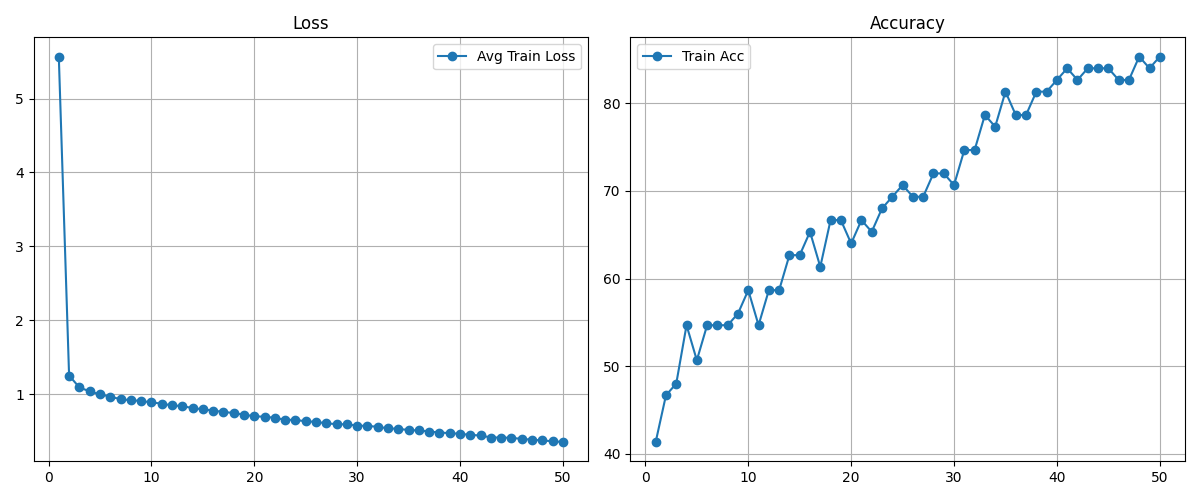
\includegraphics[width=\columnwidth]{mnist_train_stats.png} 
    \caption{Training Loss and Accuracy per epoch for MNIST three-class subset.}
    \label{fig:training_plots} 
\end{figure}

The confusion matrix for the test set predictions is shown in Fig. \ref{fig:confusion_matrix}.

\begin{figure}[!ht]
    \centering
    % Replace with the actual path to your confusion matrix image
    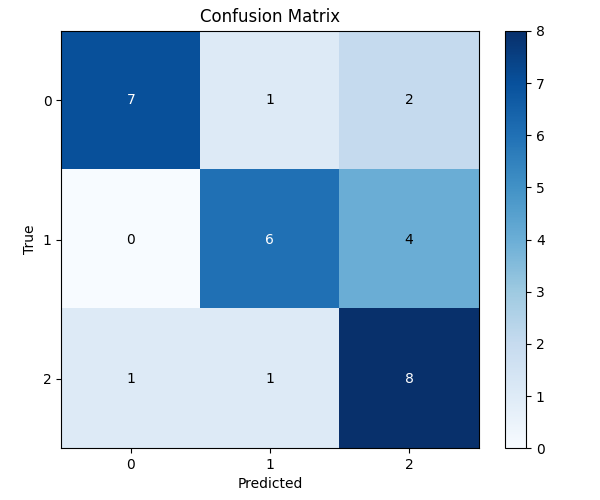
\includegraphics[width=0.8\columnwidth]{mnist_confusion_matrix.png} 
    \caption{Confusion Matrix on the MNIST three-class test subset.}
    \label{fig:confusion_matrix}
\end{figure}

\subsection{Discussion}
The model achieved an accuracy of 70\% on the test set, which is a good performance. This suggests that the whole network is indeed trainable and predictable for this simplified task. From the per-class metrics, class '0' has the highest precision while class '2' has the highest recall. Besides, the confusion matrix (Fig. \ref{fig:confusion_matrix}) provides further insight about misclassifications where class '1' was sometimes confused with class '2'.

The critical limitation of this from-scratch implementation could be the inefficiency in computation due to the repetitive use of Python lists and loops for algorithms which use a lot of memory. Furthermore, the backpropagation for the convolutional layer, especially the calculation of the gradient with respect to its input, was simply implemented and only suitable for stride = 1. Therefore, this may not fit more general convolutional parameters without careful derivation. In addition, this simple version of CNN cannot be used for a complex dataset. An experiment was carried out with the full MNIST dataset and the result was not positive: the accuracy is only around 10\% after the training, which means the network did not work at all in that problem. 

\section{Conclusion}
To sum up, this project successfully demonstrated the implementation of a Convolutional Neural Network from scratch, covering essential layers including Conv2D, ReLU, MaxPool2D, Flatten, Dense, and Softmax with Cross-Entropy loss. The network was trained on a three-class subset of the MNIST dataset and achieved a test accuracy of 70\%, indicating that the feedforward and backward propagation mechanisms are capable of learning with a relatively small dataset.

The implementation process provides valuable educational insight into the cores of CNNs. Future work for this could involve optimizing the Python code, implementing proper gradient calculations for the convolutional layer, or making it adaptable for more complex dataset.

\end{document}